\documentclass[10pt, notes]{beamer}
%\documentclass[10pt, notes]{beamer}
\usepackage[utf8]{inputenc}
\usepackage[T1]{fontenc}
\usepackage{lmodern}
\usepackage{microtype}
\usepackage[]{amsmath}
\usepackage{amssymb}
\usepackage{amsfonts}
\usepackage{appendixnumberbeamer}
\usepackage[czech]{babel}
\usepackage[]{hyperref}
\usepackage{booktabs}
\usepackage[]{graphicx}
\usepackage{siunitx}
\usepackage[figurename=]{caption}
%\newcommand{\obr}[1]{Obr. převzat z \cite[#1]}
\usepackage[
    backend=biber
    ,style=iso-numeric
    ,autolang=other
    ,pagetotal=true
    ,sortlocale=cs_CZ
    ,bibencoding=UTF8
    ,spacecolon=false
    ,block=space
]{biblatex}
\addbibresource{citace.bib}

\usetheme[sectionpage=none, numbering=fraction, progressbar= head, block=fill]{metropolis}
\setbeamerfont{note page}{size=\footnotesize}
\author{Michal Šesták}
\title{Infrazvuk}
\subtitle{FNEI}
\institute{}
%\institute{Fakulta jaderná a fyzikálně inženýrská, ČVUT v Praze\\[0.5em]
%Vedoucí práce: Ing. Iva Ambrožová, Ph. D.}
\date{5. 12. 2018}
\begin{document}

\renewcommand{\figurename}{Obr.}
\renewcommand{\tablename}{Tab.}

\maketitle

%\begin{frame}{Obsah}
    %\tableofcontents
%\end{frame}

\begin{frame}
    \begin{itemize}
        \item $f< \SI{20}{Hz}$ 
        \item \textbf{Zdroje} zemětřesení, dopadající meteority, sopky, vodopády, velké vlny, počasí, zvířata, jaderné exploze, vibrující trubky \dots
        \item \textbf{Vnímání člověkem} tlak v uších i jinde (záleží na intenzitě zvuku), bolesti hlavy, nevolnosti, noční děsy, poruchy spánku, závratě 
        \item \textbf{Využití} monitorování přírodních katastrof; lokalizování ropy a plynu; předpovídání počasí; studium srdce (Balistokardiografie and Seismokardiografie)
        \item \textbf{Kde se je nevyplatí používat} sonar

    \end{itemize}
\end{frame}

\note[itemize]{
\item \textbf{Co to je} Infrasonics, vibrational or stress waves in elastic media, having a frequency below those of sound waves that can be detected by the human ear—i.e., below 20 hertz. The range of frequencies extends down to geologic vibrations that complete one cycle in 100 seconds or longer.
\item \emph{Infrasound is characterized by an ability to cover long distances and get around obstacles with little dissipation.}
\item \textbf{Zvířata} “Elephants, in particular, produce infrasound waves that travel through solid ground and are sensed by other herds using their feet, although they may be separated by hundreds of kilometres.”
\item Zvířata dokážou rozeznat blížící se přírodní katastrofu
\item \textbf{duchové} If infrasound hits at just the right strength and frequency, it can resonate with human eyes, causing them to vibrate. This can lead to distorted vision and the possibility of “ghost” sightings. Or, at least, what some would call ghost sightings. Infrasound may also cause a person to “feel” that there’s an entity in the room with him or her, accompanied by that aforementioned sense of dread.
}
\note[itemize]{
\item \textbf{ropa atd} Distinctive rock formations in which these minerals are likely to be found can be identified by sonic ranging, primarily at infrasonic frequencies. With an array of seismic detectors, a computational form of holography may be achieved.
}

\begin{frame}{Frequency range of hearing for humans and other selected animals}
    \begin{table}
        \footnotesize
        \caption{\cite{britannica}}
        \begin{tabular}{lll}
            \toprule
            &\multicolumn{2}{l}{frequency (Hz)}\\
            animal &  low& 	high\\
            \midrule
            humans      &20 	&20 000 \\
            cats        &100 	&32 000 \\
            dogs        &40 	&46 000 \\
            horses      &31 	&40 000 \\
          elephants     &16 	&12 000 \\
            cattle      &16 	&40 000 \\
            bats        &1 000 	&150 000\\
grasshoppers and locusts&100 	&50 000 \\
            rodents 	&1 000 	&100 000\\
whales and dolphins 	&70 	&150 000\\
seals and sea lions 	&200 	&55 000 \\
            \bottomrule
        \end{tabular}
    \end{table}
\end{frame}

\note[itemize]{
\item grasshoppers and locusts=kobylky a sarančata 
\item rodents=hlodavci
\item It is believed by many zoologists that this sensitivity in animals such as elephants may be helpful in providing them with early warning of earthquakes and weather disturbances. It has been suggested that the sensitivity of birds to infrasound aids their navigation and even affects their migration.
}                 	

\begin{frame}{Detekce infrazvuku}
    
\end{frame}

\begin{frame}{Monitorování zemětřesení, výzkum vnitřní stavby Země}
    \begin{columns}
        \begin{column}{0.6\textwidth}
            \begin{itemize}
                \item Cca 30 \% uvolněné energie při zemětřesení na seismické vlny
                \item P-vlny, S-vlny, povrchové vlny (destruktivní)
                \item Varovné systémy využívají P-vln
            \end{itemize}
            \begin{figure}[h]
                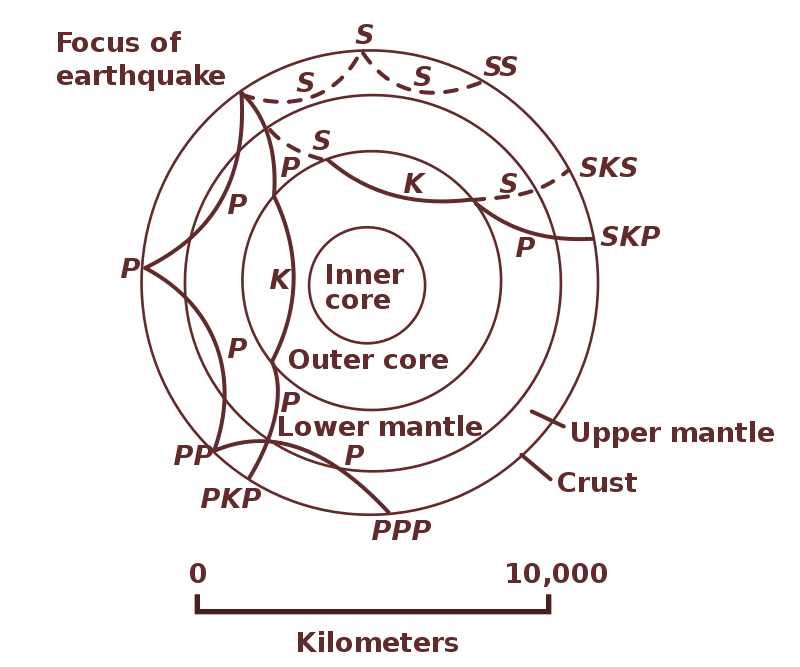
\includegraphics[width=.65\textwidth]{wave_path.png}
            \end{figure}
        \end{column}
        \begin{column}{0.4\textwidth}
            \begin{figure}
                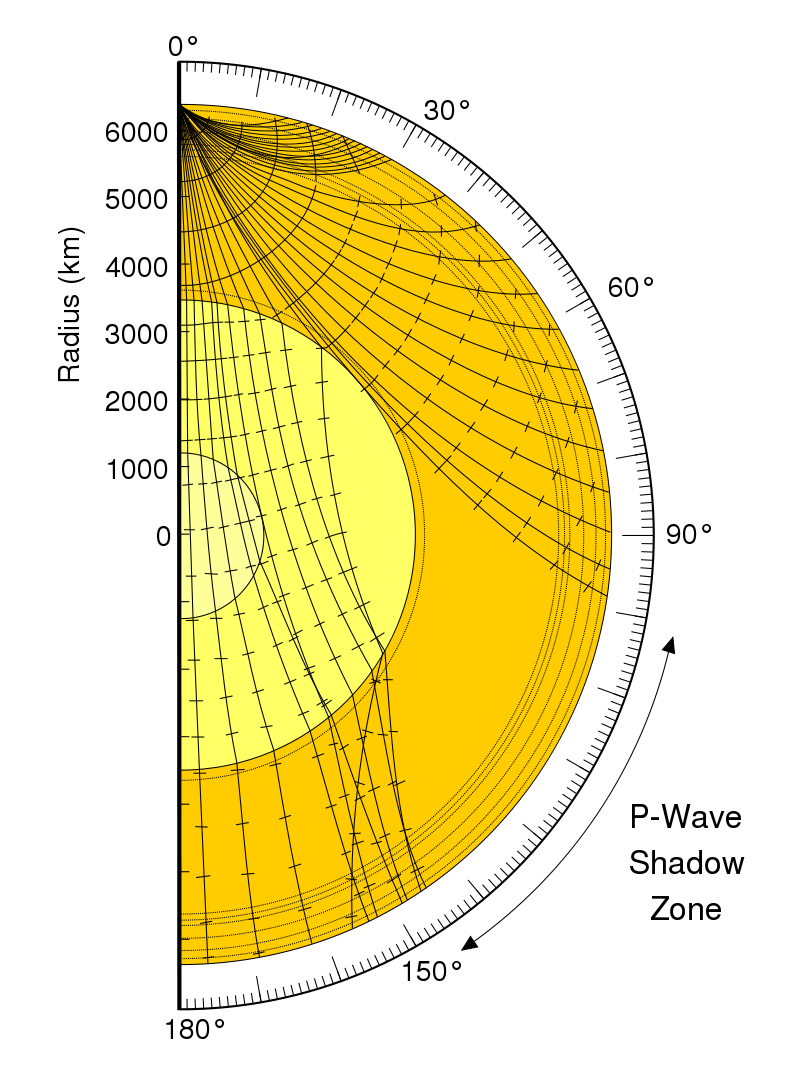
\includegraphics[width=\textwidth]{shadow_zone.png}
            \end{figure}
        \end{column}
    \end{columns}
\end{frame}

\note[itemize]{
\item P-waves (primary) se šíří rychlostí zvuku (poté co vyjdou na vzduch); S-waves (secondary) pomalejší (o cca polovinu) a příčné a pouze v pevných látkách; surface waves jsou pomalejší než oboje dvoje, cestují kolem povrchu Země, dál od povrchu mizí (propagují se na rozhraní dvou médií), dále se dělí na Love waves (L-waves, příčné) a Rayleigh waves (příčné i podélné), při velkých zemětřesení (výbuchu) mohou oběhnout mnohokrát zeměkouli \dots
\item  Surface waves are caused when P waves and S waves come to the surface. 
\item The path that a wave takes between the focus and the observation point is often drawn as a ray diagram. An example of this is shown in a figure above. When reflections are taken into account there are an infinite number of paths that a wave can take. Each path is denoted by a set of letters that describe the trajectory and phase through the Earth. In general an upper case denotes a transmitted wave and a lower case denotes a reflected wave. The two exceptions to this seem to be "g" and "n". K is P-wave in the outer core, S is S-wave in the mantle etc
}

\note{
One of the most important examples of infrasonic waves in nature is in earthquakes. Three principal types of earthquake waves exist: the S-wave, a transverse body wave; the P-wave, a longitudinal body wave; and the L-wave, which propagates along the boundary of stratified mediums. L-waves, which are of great importance in earthquake engineering, propagate in a similar way to water waves, at low velocities that are dependent on frequency. S-waves are transverse body waves and thus can only be propagated within solid bodies such as rocks. P-waves are longitudinal waves similar to sound waves; they propagate at the speed of sound and have large ranges.

When P-waves propagating from the epicentre of an earthquake reach the surface of the Earth, they are converted into L-waves, which may then damage surface structures. The great range of P-waves makes them useful in identifying earthquakes from observation points a great distance from the epicentre. In many cases, the most severe shock from an earthquake is preceded by smaller shocks, which can be detected by seismographs and provide advance warning of the greater shock to come. Underground nuclear explosions also produce P-waves, allowing them to be monitored from any point in the world if they are of sufficient intensity.}
\note{The development of extremely sensitive detectors to monitor such explosions has contributed to the maintenance of the Nuclear Test-Ban Treaty, which was signed in 1963 and banned all tests of nuclear weapons except those conducted underground so as to limit the amount of radioactive fallout in the atmosphere.

Infrasonic disturbances of the atmosphere that may extend to 50 km (30 miles) above Earth’s surface are often associated with severe earthquakes. These waves can travel considerable distances around the globe.}

\begin{frame}{Počasí}
    \begin{itemize}
        \item Monitorování stratosféry pomocí infrazvuku -> potenciálně lepší předpovědi počasí
        \item Předpovídání tornád 
            \begin{figure}[h]
                \centering
                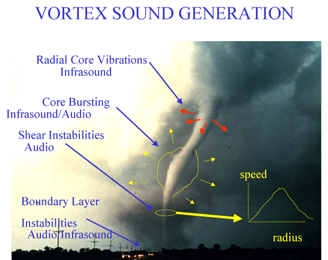
\includegraphics[width=.45\textwidth]{tornado.png}
            \end{figure}
    \end{itemize}
    \cite{weather, tornado, tornado2}
\end{frame}

\note[itemize]{
\item monitorování stratosféry i předpovídání tornád jsou nové nápady (z roku 2018)
}
\note{
This is of particular importance during a particular weather phenomenon, the sudden stratospheric warming (SSW), explains Smets. In mid-February such an event was responsible for the coldest week of this winter in the Netherlands. "Such a sudden warming of the stratosphere is an important characteristic of the winter atmosphere in the northern hemisphere. During this short-lived phenomenon the stratosphere exerts a strong influence on the layer beneath it, the troposphere. This has consequences for the weather and for weather forecasts. In recent years attempts have been made to improve predicting the stratospheric variability using numerical weather forecasts. However, this requires extra independent observations of the upper atmosphere, and this is an area that is extremely difficult to observe. Wind observations, for example, are lacking in weather models past the middle of the stratosphere, higher than around 30 km."

Read more at: \url{https://phys.org/news/2018-03-inaudible-infrasound-weather-climate.html}
}

\begin{frame}
    TO DO:

    \url{https://phys.org/news/2018-03-volcanic-eruptions.html}
\end{frame}

% různá nastavení
%\metroset{sectionpage=simple,none}
%\begin{overlayarea}{\textwidth}{\textheight}\end{overlayarea}


\begin{frame}{Reference}
    \nocite{*}
\renewcommand*{\bibfont}{\tiny}
\printbibliography
\end{frame}
\end{document}
